\section{C++多线程编程}
\subsection{开辟线程}
多线程编程主要为了解决程序中的并发问题,计算机术语中的"并发",指的是在单个系统里同时执行多个独立的活动,而不是顺序的一个接一个的执行。对于单核CPU来说,在某个时刻只可能处理一个任务,但它却不是完全执行完一个任务再执行一个下一任务,而是一直在任务间切换,每个任务完成一点就去执行下一个任务,看起来就像任务在并行发生,虽然不是严格的同时执行多个任务,但是我们仍然称之为并发(concurrency)。真正的并发是在在多核CPU上,能够真正的同时执行多个任务,称为硬件并发(hardware concurrency)。

C++处理并发任务的方式包括进程并发和线程并发两种;进程并发更为安全,可部署在分布式系统上,但通信机制较为复杂,需要耗费更多的系统资源;线程并发基于共享内存实现,由于线程间的大量数据可以共享,线程并发具有更小的资源消耗和运行速度,但同时也需要更为范围的程序语言维护以防出错。图\ref{fig.concurrenncy}给出了进程并发于线程并发的区别。
\begin{figure}[htbp]
	\centering
	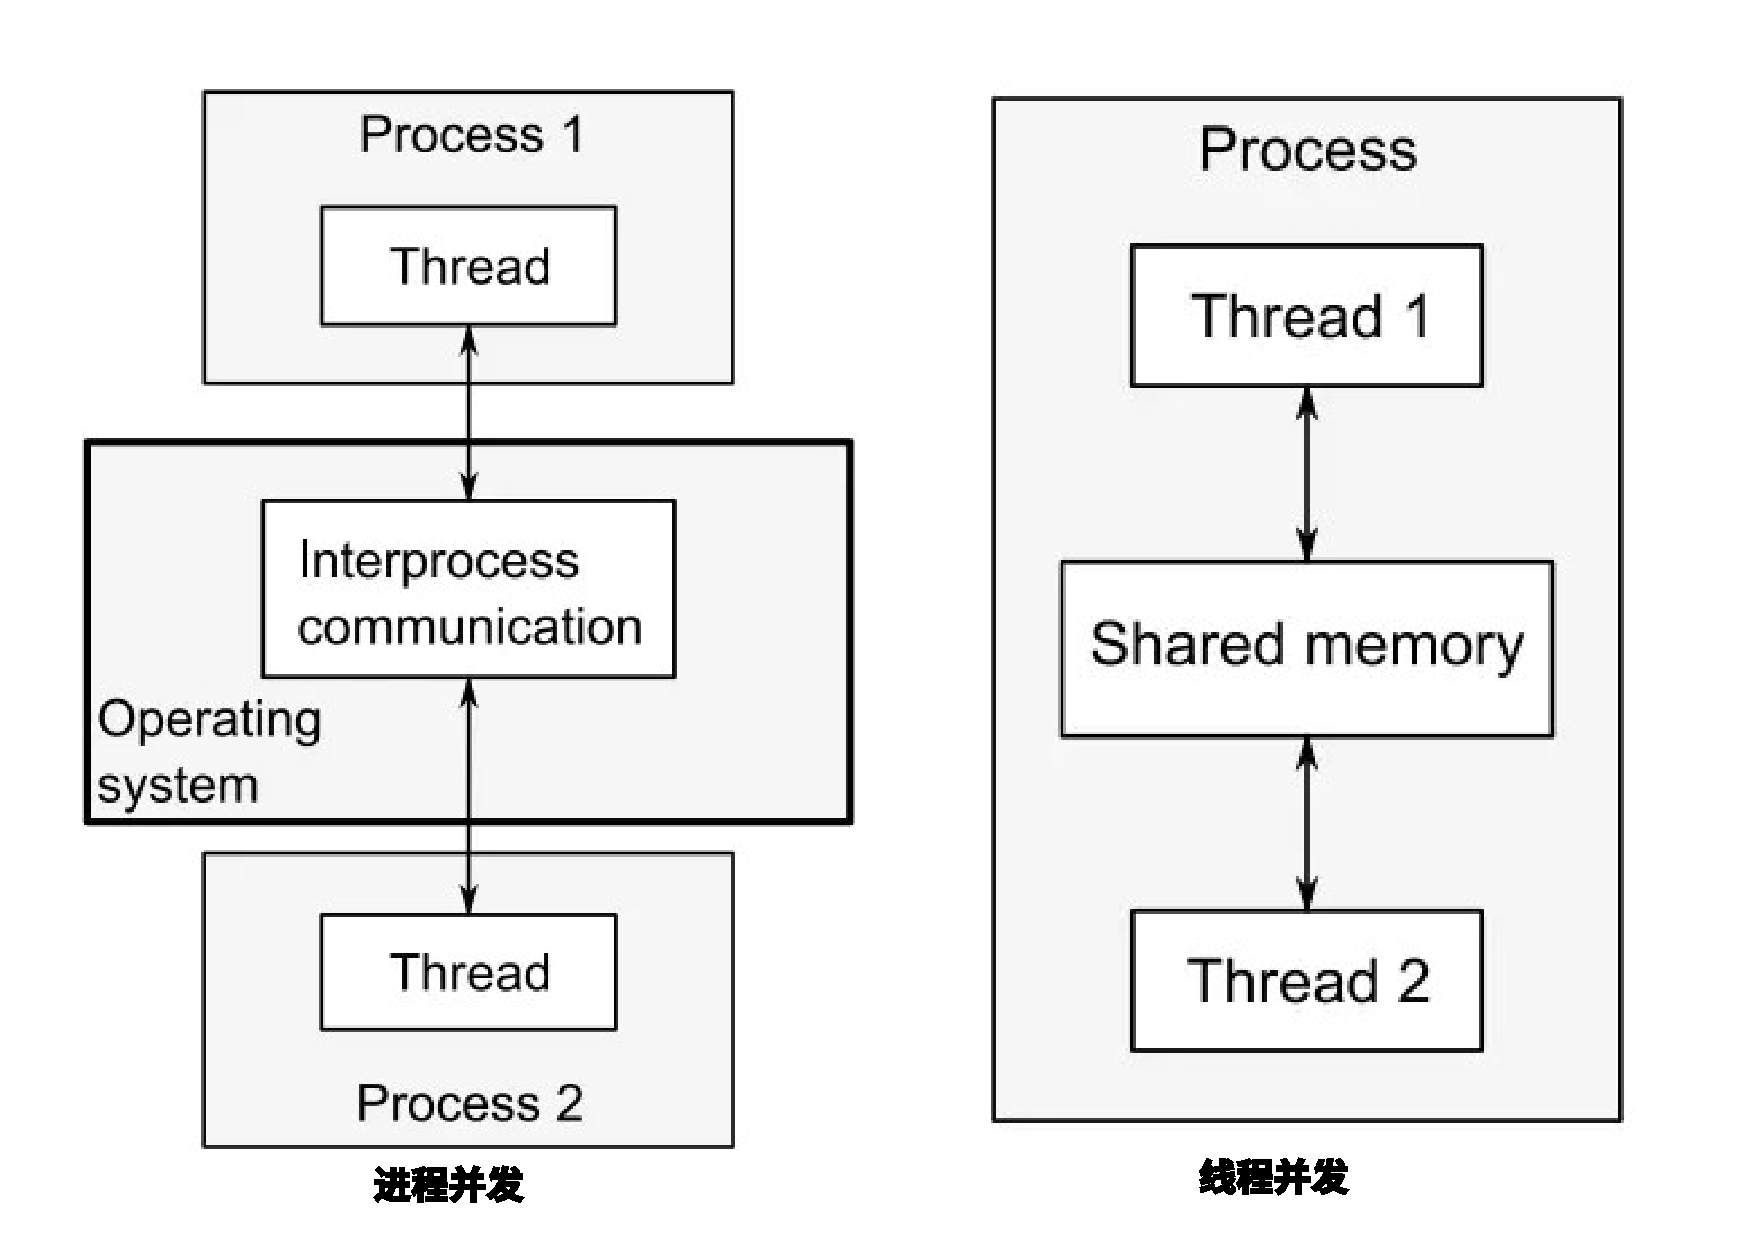
\includegraphics[scale=0.5]{Concurrency}
	\caption{进程并发与线程并发}
	\label{fig.concurrenncy}
\end{figure}
C++98标准中并没有线程库的存在,而在C++11中终于提供了多线程的标准库,提供了管理线程、保护共享数据、线程间同步操作、原子操作等类。多线程库对应的头文件是<\textbf{thread}>,类名为\textbf{std::thread}。现在假设我们有一个函数function1(),单线程串行运行该程序的代码为:\\
\begin{lstlisting}
#include <iostream>
#include <thread>

void function_1() {
	std::cout << "I'm function_1()" << std::endl;
}

int main() {
	function_1();
	return 0;
}
\end{lstlisting}
这里我们并没有使用thread的相关功能去开辟和管理线程,这是因为main()函数本身即为一个线程,成为主线程,所有的程序会在主线程中顺序运行。若我们向让function1()在其他线程中运行,可以按如下方式改写:\\
\begin{lstlisting}
#include <iostream>
#include <thread>

void function_1() {
	std::cout << "I'm function_1()" << std::endl;
}

int main() {
	std::thread t1(function_1);//开辟一个线程t1并运行函数function1
	// do other things
	std::cout << "main() before" << std::endl;
	std::cout << "main() before" << std::endl;
	std::cout << "main() before:" << std::endl;
	t1.join();//
	std::cout << "main() after" << std::endl;
	return 0;
}
\end{lstlisting}
代码分析:
\begin{enumerate}
	\item 首先使用std::thread name(fcn)函数创建一个\textbf{线程对象},fcn称为线程对象的\textbf{入口函数},该函数的运行周期即为线程的生命周期。
	\item 当线程对象t1创建后,对应的线程函数function1()即开始同步运行,函数运行结束即标志着\textbf{线程}结束,但\textbf{线程对象}并未释放;
	\item main线程和t1线程是同步执行的,但两个线程并不是同时结束的,因此需要在main函数中设定线程的执行类型。线程的类型包括join()和detach()两种;join()称为线程等待函数,main线程在同步运行至join()函数时,会判断对应的t1线程是否运行完成;若完成子继续运行main线程中join()后的内容,否则等待t1线程运行。与之相对,detach()称为线程分离函数,main线程运行至detach()时会将t1线程分离出去,随即继续运行main线程的后续内容。
\end{enumerate}
\subsection{线程构造函数}
线程构造函数std::thread()是一个可变参数函数,第一个参数为线程的入口函数,后面参数以此为入口函数的对应参数,例如:
\begin{lstlisting}
// 普通函数 无参
void function_1() {
}

// 普通函数 1个参数
void function_2(int i) {
}

// 普通函数 2个参数
void function_3(int i, std::string m) {
}

std::thread t1(function_1);
std::thread t2(function_2, 1);
std::thread t3(function_3, 1, "hello");

t1.join();
t2.join();
t3.join();
\end{lstlisting}
需要注意的是,线程的入口函数不接受重载函数,重载函数会使得编译器无法决定正确的函数类型从而引发编译错误。

此外,入口函数还可以是仿函数、匿名函数和std::function对象。
\begin{enumerate}
	\item 仿函数:
	\begin{lstlisting}
		// 仿函数
		class Fctor {
		public:
		// 具有一个参数
		void operator() () {
		
		}
		};
		Fctor f;
		std::thread t1(f);  
		// std::thread t2(Fctor()); // 编译错误 
		std::thread t3((Fctor())); // ok
		std::thread t4{Fctor()}; // ok
	\end{lstlisting}
	\item 匿名函数:
	\begin{lstlisting}
		std::thread t1([](){
		std::cout << "hello" << std::endl;
		});
		
		std::thread t2([](std::string m){
		std::cout << "hello " << m << std::endl;
		}, "world");
	\end{lstlisting}
	\item std::function:
	\begin{lstlisting}
		class A{
		public:
		void func1(){
		}
		
		void func2(int i){
		}
		void func3(int i, int j){
		}
		};
		
		A a;
		std::function<void(void)> f1 = std::bind(&A::func1, &a);
		std::function<void(void)> f2 = std::bind(&A::func2, &a, 1);
		std::function<void(int)> f3 = std::bind(&A::func2, &a, std::placeholders::_1);
		std::function<void(int)> f4 = std::bind(&A::func3, &a, 1, std::placeholders::_1);
		std::function<void(int, int)> f5 = std::bind(&A::func3, &a, std::placeholders::_1, std::placeholders::_2);
		
		std::thread t1(f1);
		std::thread t2(f2);
		std::thread t3(f3, 1);
		std::thread t4(f4, 1);
		std::thread t5(f5, 1, 2);
	\end{lstlisting}
\end{enumerate}

注1:需要注意的是,线程入口函数传入的参数只有\textbf{传值}一种类型,即便入口函数的参数是引用形式,为了保证线程数据的安全性,新开辟线程也会在构造线程兑现对传入的数值进行拷贝。
注2:线程对象之间是不能复制的,只能移动,移动的意思是,将线程的所有权在std::thread实例间进行转移。
\begin{lstlisting}
	void some_function();
	void some_other_function();
	std::thread t1(some_function);
	// std::thread t2 = t1; // 编译错误
	std::thread t2 = std::move(t1); //只能移动 t1内部已经没有线程了
	t1 = std::thread(some_other_function); // 临时对象赋值 默认就是移动操作
	std::thread t3;
	t3 = std::move(t2); // t2内部已经没有线程了
	t1 = std::move(t3); // 程序将会终止,因为t1内部已经有一个线程在管理了
\end{lstlisting}
\subsection{线程与竞争条件}
并发代码中最常见的错误之一就是竞争条件(race condition)。而其中最常见的就是数据竞争(data race),从整体上来看,所有线程之间共享数据的问题,都是修改数据导致的,如果所有的共享数据都是只读的,就不会发生问题。但是这是不可能的,大部分共享数据都是要被修改的。

std::cout()就是一个典型的共享资源对象,其操作基于数据流实现:\\
\begin{lstlisting}
#include <iostream>
#include <thread>
#include <string>
using namespace std;

// 普通函数 无参
void function_1() {
for(int i=0; i>-100; i--)
	cout << "From t1: " << i << endl;
}

int main()
{
	std::thread t1(function_1);
	
	for(int i=0; i<100; i++)
		cout << "From main: " << i << endl;
	
	t1.join();
	return 0;
}
\end{lstlisting}
在上面这里demo中,运行结果会出现如下的混乱情况,这是因为cout的数据流在两个线程中是共享的,两个线程执行cout取出数据的时机是完全随机的:\\
\begin{lstlisting}
From main: 0
From main: 1From t1: 
From main: 2
\end{lstlisting}
c++中提供了解决这一问题的方式——互斥锁(Mutex),其包含在头文件<\textbf{mutex}>中,在使用共享资源前使用std::mutex.lock()锁定线程,使用完毕后使用std::mutex.unlock()解锁线程,即可保护共享资源对象:\\
\begin{lstlisting}
#include <iostream>
#include <thread>
#include <string>
#include <mutex>
using namespace std;

std::mutex mu;
// 使用锁保护
void shared_print(string msg, int id) {
	mu.lock(); // 上锁
	cout << msg << id << endl;
	mu.unlock(); // 解锁
}

void function_1() {
	for(int i=0; i>-100; i--)
		shared_print(string("From t1: "), i);
}

int main()
{
	std::thread t1(function_1);
	
	for(int i=0; i<100; i++)
		shared_print(string("From main: "), i);
	
	t1.join();
	return 0;
}	
\end{lstlisting}
但由用户手动加锁与解锁存在一个隐藏问题,即当lock于unlock之间的代码出现异常退出时,系统不会自动将共享资源解锁,时候后续需要使用该共享资源的线程秩序堵塞。C++标准库提供了lock\_guard模板类解决这一问题,该模板类是c++中常见的RAII技术,即获取资源即初始化(Resource Acquisition Is Initialization)技术。该模板类在创建类对象的时候会自动对线程加锁,在对象析构时,则会自动对线程解锁。\\
\begin{lstlisting}
void shared_print(string msg, int id) {
	//构造的时候帮忙上锁
	std::lock_guard<std::mutex> guard(mu);
	
	cout << msg << id << endl;
	//即便代码出现异常退出,由于函数运行结束,函数内创建的lock_guard对象
	//释放时会自动调用析构函数,保证线程解锁
}
\end{lstlisting}
同时,由于mutex本身是一个全局变量,但其服务对象仅为shared\_print函数,因此可以将两者分别封装为类的成员变量和成员函数,以优化代码:\\
\begin{lstlisting}
#include <iostream>
#include <thread>
#include <string>
#include <mutex>
#include <fstream>
using namespace std;

std::mutex mu;
class LogFile {
std::mutex m_mutex;
ofstream f;
public:
LogFile() {
f.open("log.txt");
}
~LogFile() {
f.close();
}
void shared_print(string msg, int id) {
std::lock_guard<std::mutex> guard(mu);
f << msg << id << endl;
}
};

void function_1(LogFile& log) {
for(int i=0; i>-100; i--)
log.shared_print(string("From t1: "), i);
}

int main()
{
LogFile log;
//log对象不能拷贝,需要使用ref传入原引用
std::thread t1(function_1, std::ref(log));

for(int i=0; i<100; i++)
log.shared_print(string("From main: "), i);

t1.join();
return 0;
}
\end{lstlisting}
上一节我们提到过,线程函数的参数本质是拷贝而非赋值。这里由于ofstream对象不能直接拷贝,需要使用std::ref()函数将原对象的引用传入。
\subsection{死锁}
将mutex上锁而不解锁的情况称为\textbf{死锁},这种情况下使用lock\_guard可以保证析构的时候能够释放锁,然而,当一个操作需要使用两个互斥锁的时候,仅仅使用lock\_guard并不能保证不会发生死锁,如下面的例子:
\begin{lstlisting}
#include <iostream>
#include <thread>
#include <string>
#include <mutex>
#include <fstream>
using namespace std;

class LogFile {
	std::mutex _mu;
	std::mutex _mu2;
	ofstream f;
public:
	LogFile() {
		f.open("log.txt");
	}
	~LogFile() {
		f.close();
	}
	void shared_print(string msg, int id) {
		std::lock_guard<std::mutex> guard(_mu);
		std::lock_guard<std::mutex> guard2(_mu2);
		f << msg << id << endl;
		cout << msg << id << endl;
	}
	void shared_print2(string msg, int id) {
		std::lock_guard<std::mutex> guard(_mu2);
		std::lock_guard<std::mutex> guard2(_mu);
		f << msg << id << endl;
		cout << msg << id << endl;
	}
};

void function_1(LogFile& log) {
	for(int i=0; i>-100; i--)
		log.shared_print2(string("From t1: "), i);
}

int main()
{
	LogFile log;
	std::thread t1(function_1, std::ref(log));
	
	for(int i=0; i<100; i++)
		log.shared_print(string("From main: "), i);
	
	t1.join();
	return 0;
}
\end{lstlisting}
该demo中由于同时使用了两个互斥锁,在某些状况下会出现嵌套死锁,应尽量避免。
\subsection{unique\_lock}
使用互斥锁虽然保证了共享数据的唯一性,但亦将并行操作变为了串行操作,降低了代码效率,因此需要谨慎的设计上锁的代码块。如果一段代码中有多个代码块需要频繁的加锁与解锁,由于lock\_guard只会在创建时上锁,在析构时解锁,就需要创建多个局部lock\_guard对象,例如:\\
\begin{lstlisting}
std::mutex _mu;
{
	std::lock_guard<std::mutex> guard(_mu);
	\\code....
}
{
	std::lock_guard<std::mutex> guard(_mu);
	\\code....	
}
{
	std::lock_guard<std::mutex> guard(_mu);
	\\code....
}
\end{lstlisting}
这无疑增加了代码的复杂度,降低了可阅读性。而使用unique\_lock则可有效改善这一问题。unique\_lock提供了lock()和unlock()接口,能记录现在处于上锁还是没上锁状态,在析构的时候,会根据当前状态来决定是否要进行解锁(lock\_guard就一定会解锁)。上面的代码修改如下:\\
\begin{lstlisting}
class LogFile {
	std::mutex _mu;
	ofstream f;
	public:
		LogFile() {
			f.open("log.txt");
		}
		~LogFile() {
			f.close();
		}
		void shared_print(string msg, int id) {
		
			std::unique_lock<std::mutex> guard(_mu);
			//do something 1
			guard.unlock(); //临时解锁
			//do something 2
			guard.lock(); //继续上锁
			// do something 3
			f << msg << id << endl;
			cout << msg << id << endl;
			// 结束时析构guard会临时解锁
			// 这句话可要可不要,不写,析构的时候也会自动执行
			// guard.ulock();
	}
};
\end{lstlisting}
可以看到,unique\_lock记录了当前锁的状态,在无需加锁的代码区域,可以使用unlock借口临时解锁,随后再重新加锁。但由于需要一直维护锁的状态,unique\_lock的执行效率比lock\_guard要低,因此能使用lock\_guard解决的代码应尽量使用lock\_guard。

同时需要注意的是,lock\_guard和unique\_lock均不能复制,但unique\_lock可以移动。
\subsection{条件变量}
在C++11以后的标准中,条件变量是实现线程同步管理的另一个有效方式,其通常和unique\_lock一同配套使用以避免线程间的竞争。使用条件变量需要包含头文件\textbf{condition\_variable},其主要包括两个重要的成员函数机制,等待和唤醒:\\
\begin{enumerate}
	\item 等待 
		\iitem wait():阻塞当前线程直到条件变量唤醒
		\iitem wait\_for():阻塞当前线程直到条件变量唤醒或到达一定时间
		\iitem wait\_until():阻塞当前线程直到条件变量唤醒或到达指定时间点
	\item 唤醒
		\iitem notify\_one():随机唤醒一个等待线程
		\iitem notify\_all():唤醒所有等待线程
\end{enumerate}
其中,所有wait函数接受参数均为std::unique\_lock<std::mutex>对象,且可以选择使用微词pred避免虚假唤醒,即:\\
\begin{lstlisting}
void wait( std::unique_lock<std::mutex>& lock );
//Predicate 谓词函数,可以普通函数或者lambda表达式
template< class Predicate >
void wait( std::unique_lock<std::mutex>& lock, Predicate pred );
\end{lstlisting}